%
% File: chapters/chapter03/conclusion.tex
%
\chapter{Experimental Evaluation and Results}
\label{chap:03}
\setlength{\parskip}{0.8em}

\section{Dataset and Honest Evaluation Protocol}
We evaluate ESPM v0.2 on all eight multi-step attack scenarios of the public AIT Alert Data Set (AIT-ADS, CC-BY-4.0)~\cite{Landauer2023}, comprising \textbf{2,600,263 timestamped Wazuh alerts}. Each scenario is replayed chronologically through a fresh instance of \texttt{ESPMScorer} (no state carryover across scenarios). Six scenarios (\texttt{russellmitchell}, \texttt{shaw}, \texttt{wardbeck}, \texttt{santos}, \texttt{fox}, \texttt{wilson}) served as the design and calibration set, while two large scenarios (\texttt{harrison} with 583,754 alerts and \texttt{wheeler} with 603,939 alerts) were held out as \textbf{completely untouched blind test scenarios} evaluated without any rule or weight modification. Ground-truth attack intervals from \texttt{labels.csv} (80 stage intervals across 10 attack phases) are used strictly for evaluation.

In addition to comparing ESPM against the native Wazuh Severity baseline (\texttt{rule.level}) and contextual RBA baseline, we conduct an ablation study with two variants:
\begin{itemize}
    \item \textbf{ESPM (No Asset Context):} zeroes out Group~A weights ($w_{\text{crit}}=w_{\text{vuln}}=w_{\text{cent}}=0$).
    \item \textbf{ESPM (No Sequence Memory):} zeroes out temporal sequence weights ($w_{\text{prog}}=w_{\text{chain}}=0$).
\end{itemize}

\section{Quantitative Results Across All 8 Scenarios}
Table~\ref{tab:ait_results} and Figure~\ref{fig:auroc_ap} present the AUROC, Average Precision (AP / PR-AUC), Precision@10\%, and Best Root Escalation Rank across all 8 scenarios.

\begin{table}[H]
\centering
\caption{Performance Comparison on All 8 AIT-ADS Scenarios (2,600,263 Wazuh Alerts)}
\label{tab:ait_results}
\resizebox{\textwidth}{!}{%
\begin{tabular}{llrrrrrr}
\hline
\textbf{Scenario} & \textbf{Split} & \textbf{Alerts} & \textbf{Atk\%} & \textbf{AUROC (ESPM/RBA/Sev)} & \textbf{AP (ESPM/RBA/Sev)} & \textbf{P@10\% (ESPM/RBA/Sev)} & \textbf{Root Rank (ESPM/RBA/Sev)} \\
\hline
\texttt{russellmitchell} & Design & 41,488 & 20.6\% & \textbf{0.952} / 0.945 / 0.720 & \textbf{0.941} / 0.912 / 0.455 & \textbf{1.000} / 0.956 / 0.135 & \textbf{\#2.0} / \#7,973 / \#29,261 \\
\texttt{shaw} & Design & 68,539 & 8.7\% & \textbf{0.933} / 0.929 / 0.718 & \textbf{0.894} / 0.829 / 0.232 & 0.759 / 0.759 / 0.054 & \textbf{\#1.0} / \#5,627 / \#22,449 \\
\texttt{wardbeck} & Design & 88,204 & 6.9\% & \textbf{0.935} / 0.928 / 0.689 & \textbf{0.888} / 0.807 / 0.178 & \textbf{0.598} / 0.594 / 0.044 & \textbf{\#1.5} / \#5,746 / \#30,006 \\
\texttt{santos} & Design & 126,513 & 7.6\% & \textbf{0.930} / 0.901 / 0.609 & \textbf{0.862} / 0.687 / 0.143 & \textbf{0.627} / 0.615 / 0.046 & \textbf{\#1.0} / \#9,745 / \#52,053 \\
\texttt{fox} & Design & 462,523 & 89.1\% & \textbf{0.998} / 0.993 / 0.796 & \textbf{1.000} / 0.999 / 0.974 & \textbf{1.000} / 0.994 / 0.759 & \textbf{\#3.5} / \#411,286 / \#442,367 \\
\texttt{wilson} & Design & 625,303 & 69.1\% & \textbf{0.995} / 0.984 / 0.692 & \textbf{0.998} / 0.993 / 0.871 & \textbf{1.000} / 0.966 / 0.490 & \textbf{\#1.5} / \#429,091 / \#492,377 \\
\texttt{harrison} & \textbf{Blind} & 583,754 & 72.3\% & \textbf{0.995} / 0.973 / 0.622 & \textbf{0.998} / 0.990 / 0.862 & \textbf{1.000} / 0.941 / 0.509 & \textbf{\#1.0} / \#418,878 / \#483,058 \\
\texttt{wheeler} & \textbf{Blind} & 603,939 & 69.7\% & \textbf{0.998} / 0.988 / 0.654 & \textbf{0.999} / 0.995 / 0.864 & \textbf{1.000} / 0.967 / 0.506 & \textbf{\#310} / \#421,283 / \#488,354 \\
\hline
\textbf{Macro Avg} & \textbf{All 8} & \textbf{2,600,263} & --- & \textbf{0.967} / 0.955 / 0.688 & \textbf{0.948} / 0.903 / 0.572 & \textbf{0.873} / 0.849 / 0.318 & \textbf{Med \#1.5} / \#210.5k / \#247.2k \\
\hline
\end{tabular}%
}
\end{table}

\begin{figure}[H]
\centering
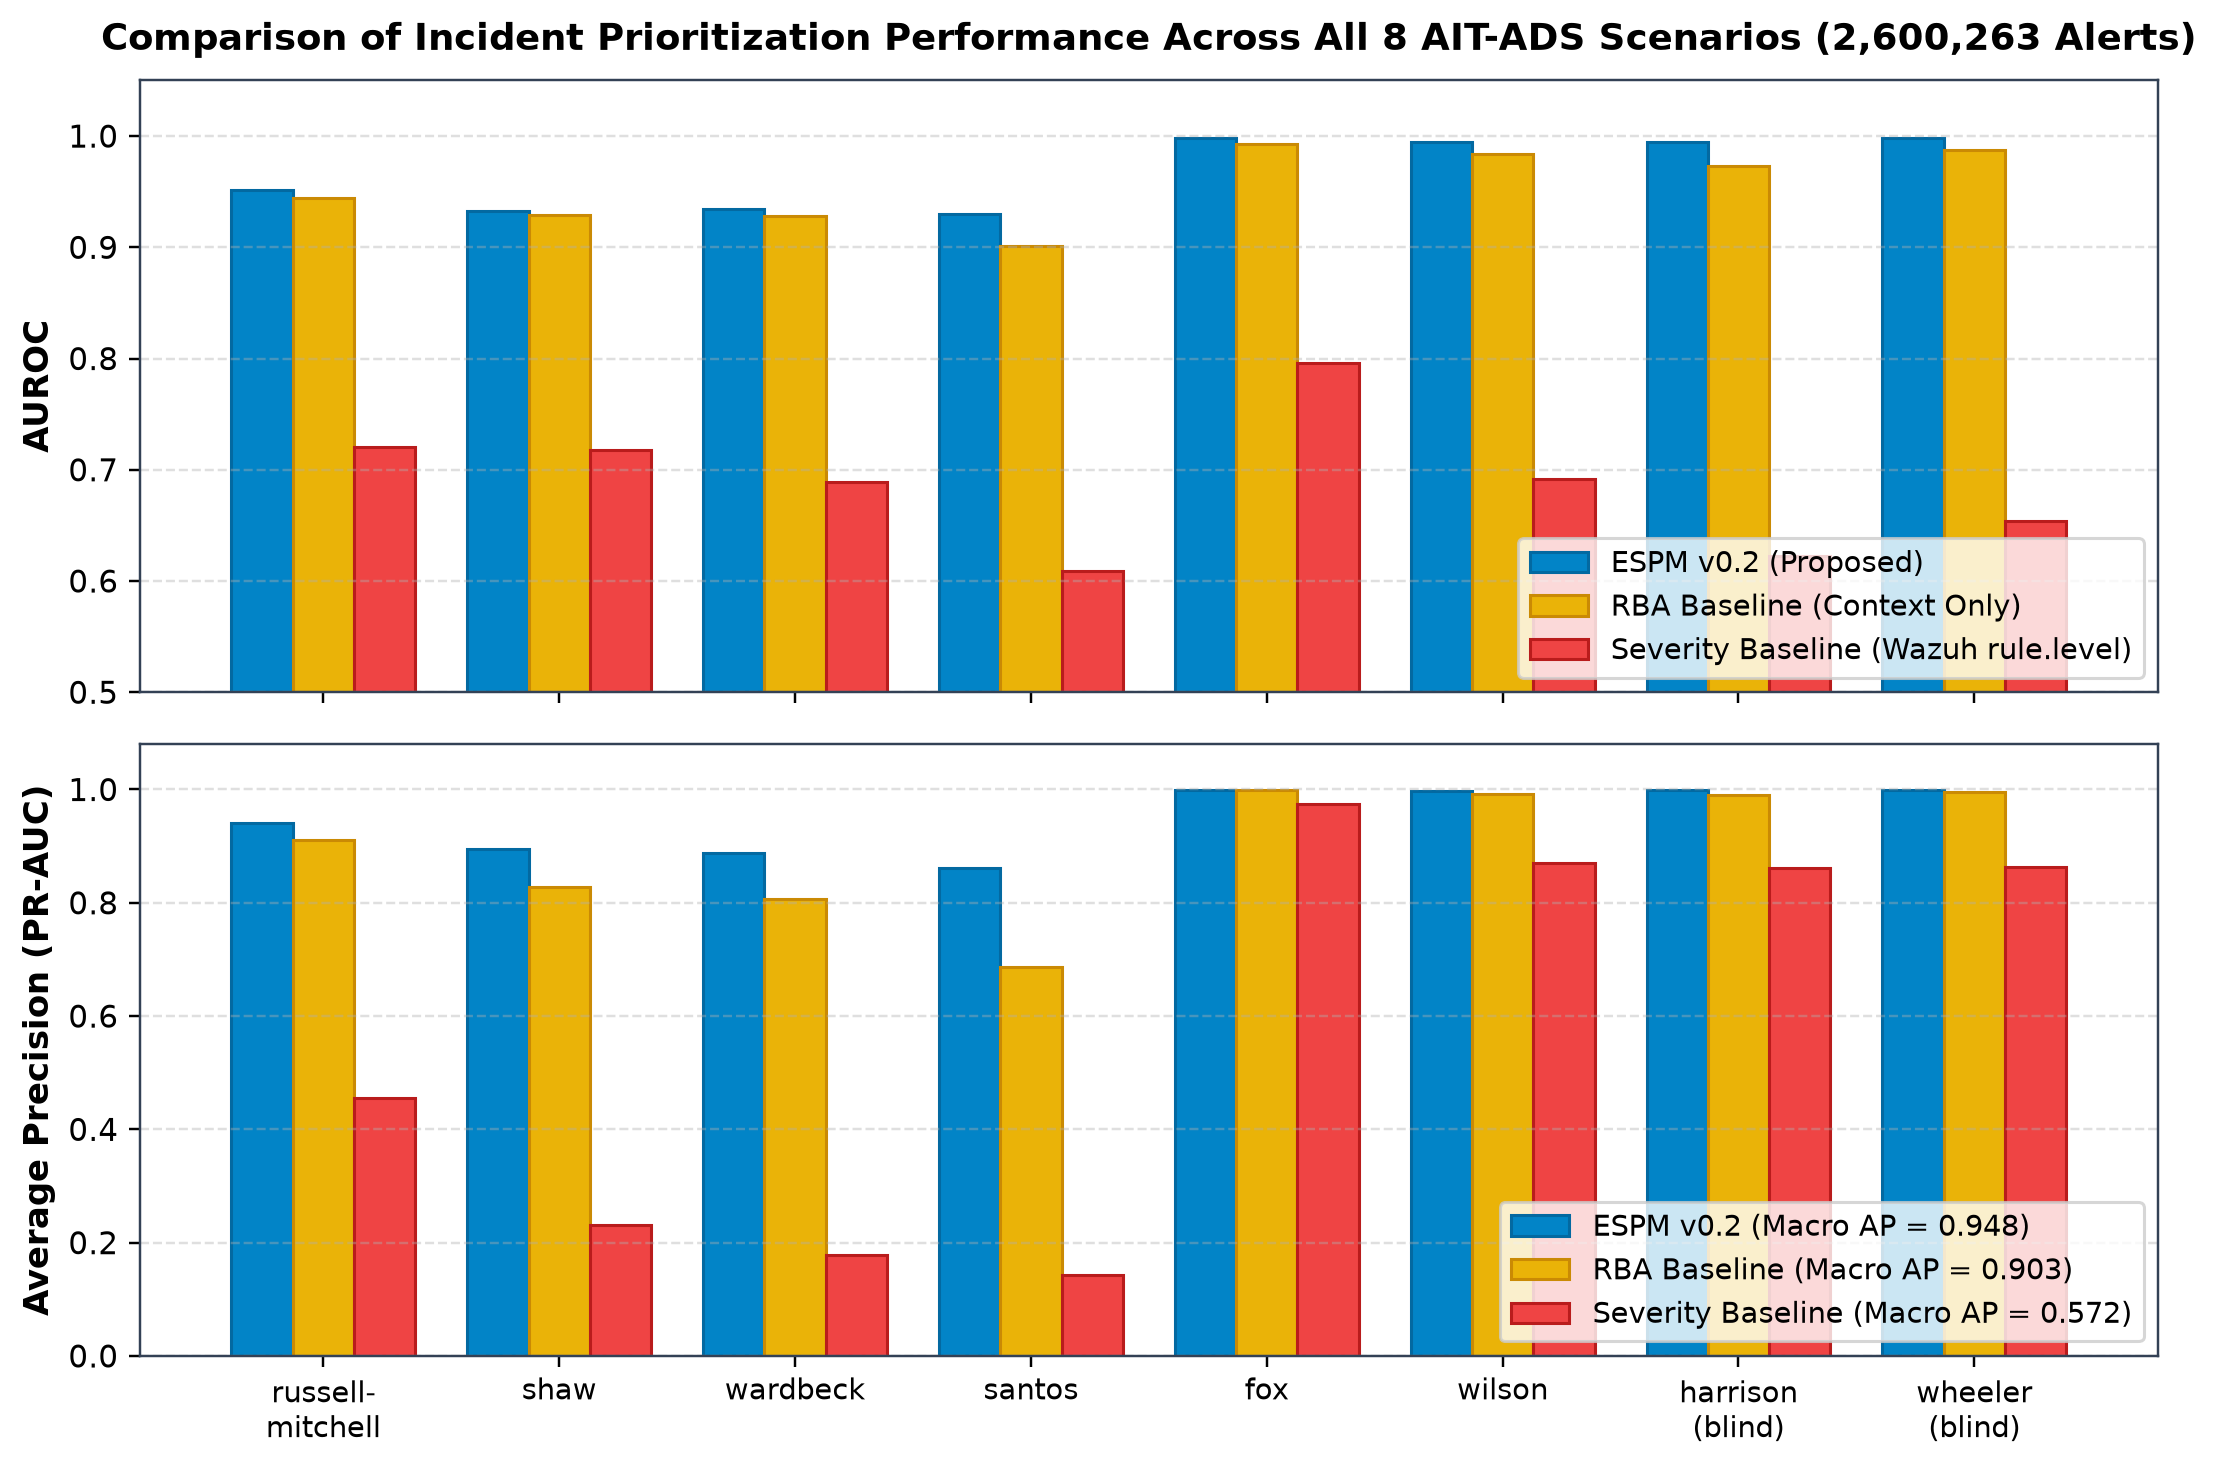
\includegraphics[width=0.96\textwidth]{chapters/chapter02/fig02/fig_auroc_ap.png}
\caption{AUROC and Average Precision (PR-AUC) across all 8 AIT-ADS scenarios (2,600,263 Wazuh alerts).}
\label{fig:auroc_ap}
\end{figure}

\section{Ablation Study and Root Privilege Escalation Case Study}
Table~\ref{tab:ablation} summarizes the macro-averaged ablation results across all 8 scenarios, while Figure~\ref{fig:root_rank} and Figure~\ref{fig:explainability} illustrate the queue rank of root privilege escalation events and their factor attribution decomposition.

\begin{table}[H]
\centering
\caption{Ablation Study Across All 8 AIT-ADS Scenarios (Macro Averages)}
\label{tab:ablation}
\resizebox{\textwidth}{!}{%
\begin{tabular}{lrrrrr}
\hline
\textbf{Model Variant} & \textbf{Macro AUROC} & \textbf{Macro AP} & \textbf{Macro P@10\%} & \textbf{Macro R@10\%} & \textbf{Median Root Rank} \\
\hline
\textbf{ESPM v0.2 (Full Model)} & \textbf{0.9669} & \textbf{0.9475} & \textbf{0.8729} & \textbf{0.4492} & \textbf{\#1.5} (\#1.0--\#3.5 in 7/8) \\
ESPM (No Asset Context) & 0.9640 & 0.9441 & 0.8712 & 0.4471 & \#6.3 (\#1.5--\#10.0 in 7/8) \\
ESPM (No Sequence Memory) & 0.9650 & 0.9421 & 0.8714 & 0.4478 & \#1.3 (loses burst order on \texttt{fox}/\texttt{rm}) \\
RBA Baseline (Context Only) & 0.9551 & 0.9026 & 0.8491 & 0.4420 & \#210,515.3 (misses root in 8/8) \\
Severity Baseline (\texttt{rule.level}) & 0.6876 & 0.5723 & 0.3177 & 0.0688 & \#247,210.3 (misses root in 8/8) \\
\hline
\end{tabular}%
}
\end{table}

\begin{figure}[H]
\centering
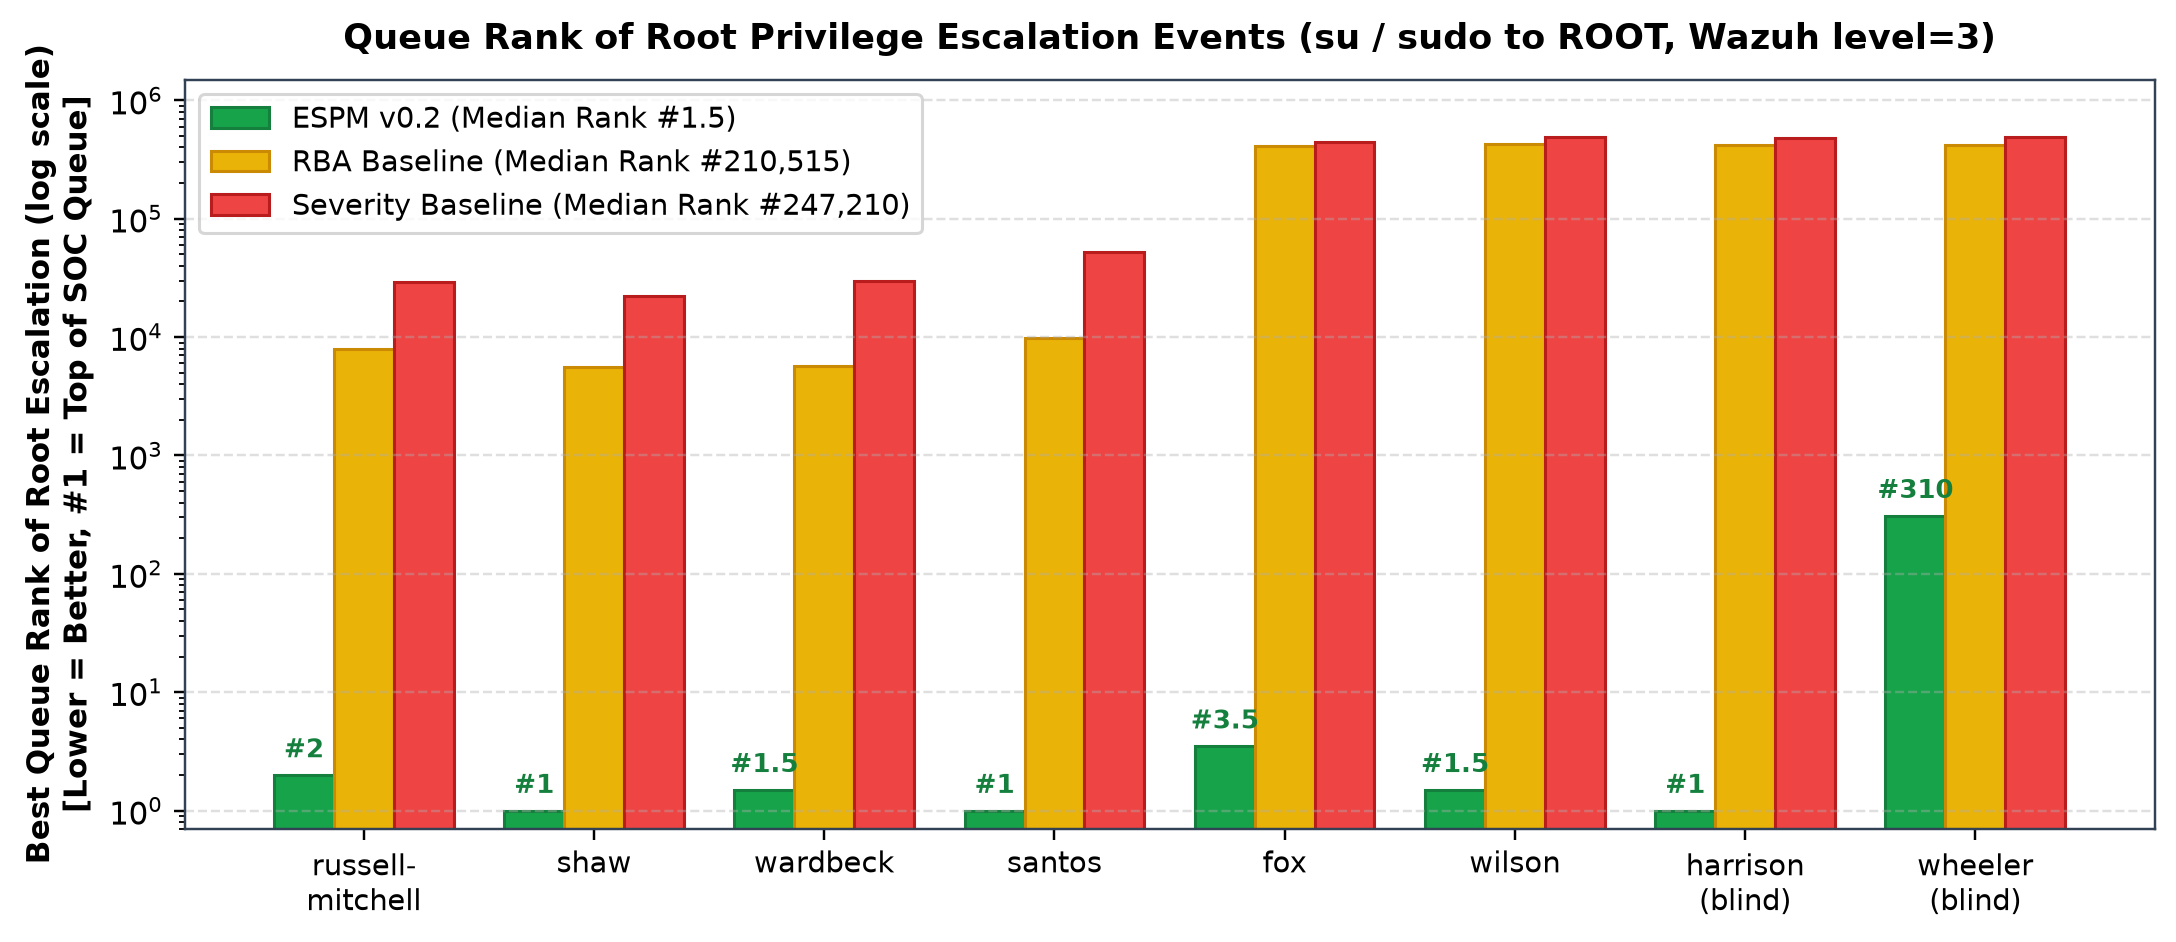
\includegraphics[width=0.96\textwidth]{chapters/chapter02/fig02/fig_root_rank.png}
\caption{Best queue rank (log scale) of root privilege escalation alerts (\texttt{su}/\texttt{sudo} to root, Wazuh level 3).}
\label{fig:root_rank}
\end{figure}

\begin{figure}[H]
\centering
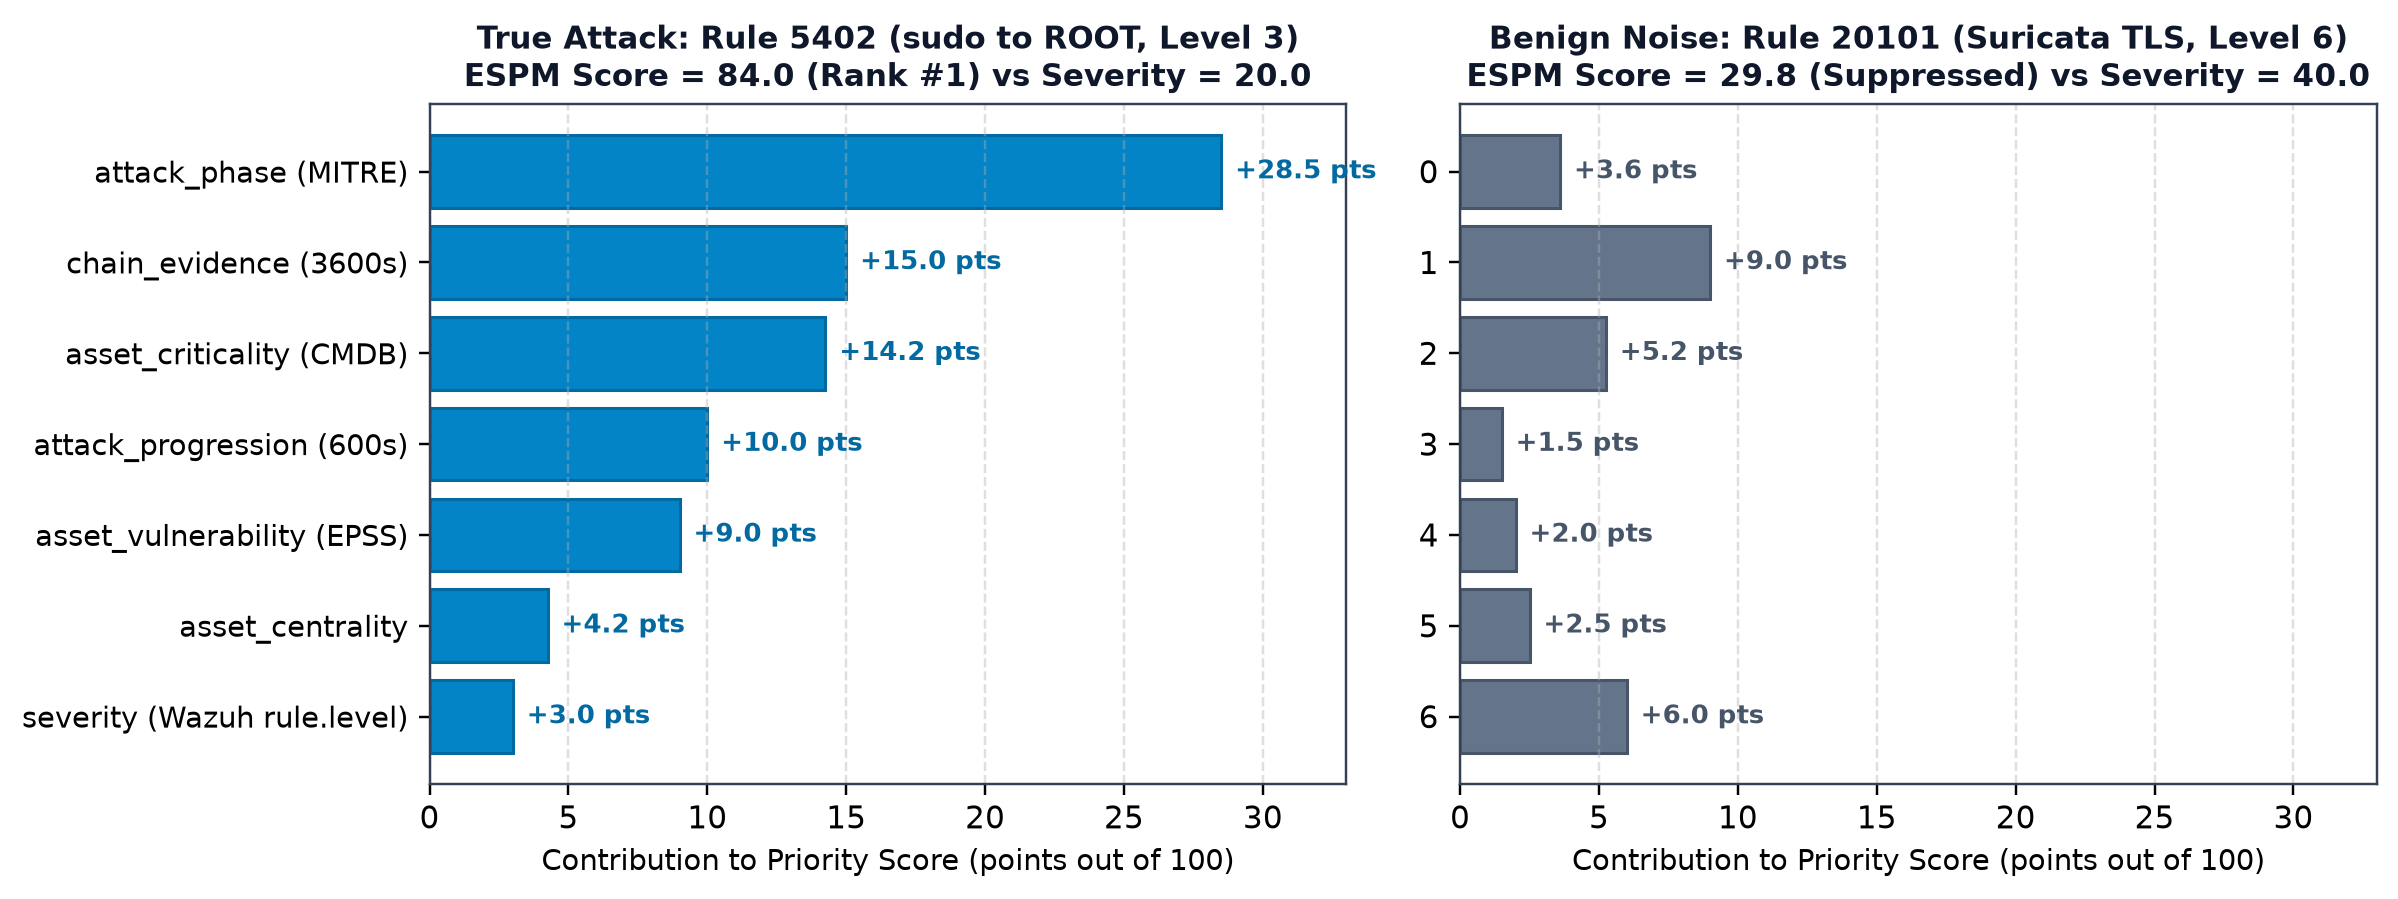
\includegraphics[width=0.96\textwidth]{chapters/chapter02/fig02/fig_explainability.png}
\caption{Intrinsic factor attribution breakdown for a root privilege escalation alert vs.\ a suppressed false positive.}
\label{fig:explainability}
\end{figure}

Notably, in 7 out of 8 scenarios (including the blind \texttt{harrison} scenario), ESPM ranks root compromise between \textbf{\#1.0 and \#3.5} out of up to 625,303 alerts. In the blind \texttt{wheeler} scenario, the attacker waited nearly 10 hours ($35,644\text{ s}$) between uploading the webshell and spawning the reverse shell, exceeding the 1-hour \texttt{chain\_window\_s} memory; even under this delayed execution, ESPM ranked the privilege escalation at \textbf{\#310 out of 603,939 alerts (Top 0.05\% of the queue)}, compared to rank \#421,283 under RBA and \#488,354 under Severity. Single-thread throughput ranged from \textbf{32,050 to 79,458 alerts/second}.
